\chapter{Configuração DNS / Bind9} \label{dns_conf}

\section{Considerações} \label{dns_intro}

Para ser possível comunicação entre os diferentes sub-sistemas da rede através dos respetivos domínios sem estarmos a depender de IPs, é necessário criar um servidor DNS.
O software escolhido foi o \textbf{BIND9}, que permite também a configuração do servidor para cache DNS.

Na estrutura de rede que estamos a analisar, temos uma rede local segura e excluída do exterior, e uma DMZ, ligada ao exterior.
Idealmente, um servidor DNS seria configurado em cada uma das zonas.
No entanto, devido a limitações de hardware, a DMZ está na mesmo \textit{host} que a rede de computadores, pelo que o servidor DNS é partilhado.
Desse modo, é preciso configurar uma \textbf{Split DNS}. Esta configuração permite a distinção dos endereços que fazem as \textit{queries}.
É assim possível fornecer uma resposta diferente dependendo do \textit{host} que está a fazer a \textit{query}.

\section{Rede de Servidores / DMZ} \label{dns_rede_servidores}

O servidor DNS na rede de servidores tem como objetivo devolver o endereço para os serviços de:
\begin{itemize}
    \item Nameserver - ns.qquma.pt
    \item Webserver - www.qquma.pt
    \item Mailserver - mail.qquma.pt
\end{itemize}

No entanto, o endereço a ser devolvido depende da origem do pedido.
Se o pedido for proveniente da rede interna (192.168.0.0/21), os endereços a devolver correspondem aos serviços alojados na rede de servidores (192.168.2.22x).
Se o pedido for externo (incluíndo da DMZ), os endereços a devolver correspondem aos serviços alojados na DMZ (20.49.51.16x).

Além disso, o servidor DNS só pode resolver pedidos para domínios da loja e do armazém a pedidos internos na rede, bloqueando pedidos externos.

Existe mais que uma forma de fazer esta separação no DNS.
A primeira, que é o exemplo fornecido pela documentação do Bind para uma \textit{Split-DNS} \cite{bind1}, faz uso das funções
\verb|allow-query{}| que especifica os endereços que permite \textit{queries} e \verb|allow-forward{}| que especifica os endereços que permite encaminhamento de \textit{queries} ao \textit{slave}.

O segundo método, que foi o escolhido, prende-se com a criação de \textit{views}, que é um conjunto de zonas que seguem as mesmas configurações gerais \cite{bind2}.
Neste caso, definimos uma \textit{view} para pedidos internos, que através da função \verb|match-clients{}| permite especificar os endereços que entram nessa \textit{view}.
Estas \textit{views} funcionam por exclusão, isto é, o pedido tenta entrar na \textit{views} por ordem e só entra na \textit{view} geral se não conseguir entrar na anterior.

Em ambos os casos, definimos ficheiros \textit{database} diferentes para as zonas internas e externas.

\begin{figure}[H]
    \centering
    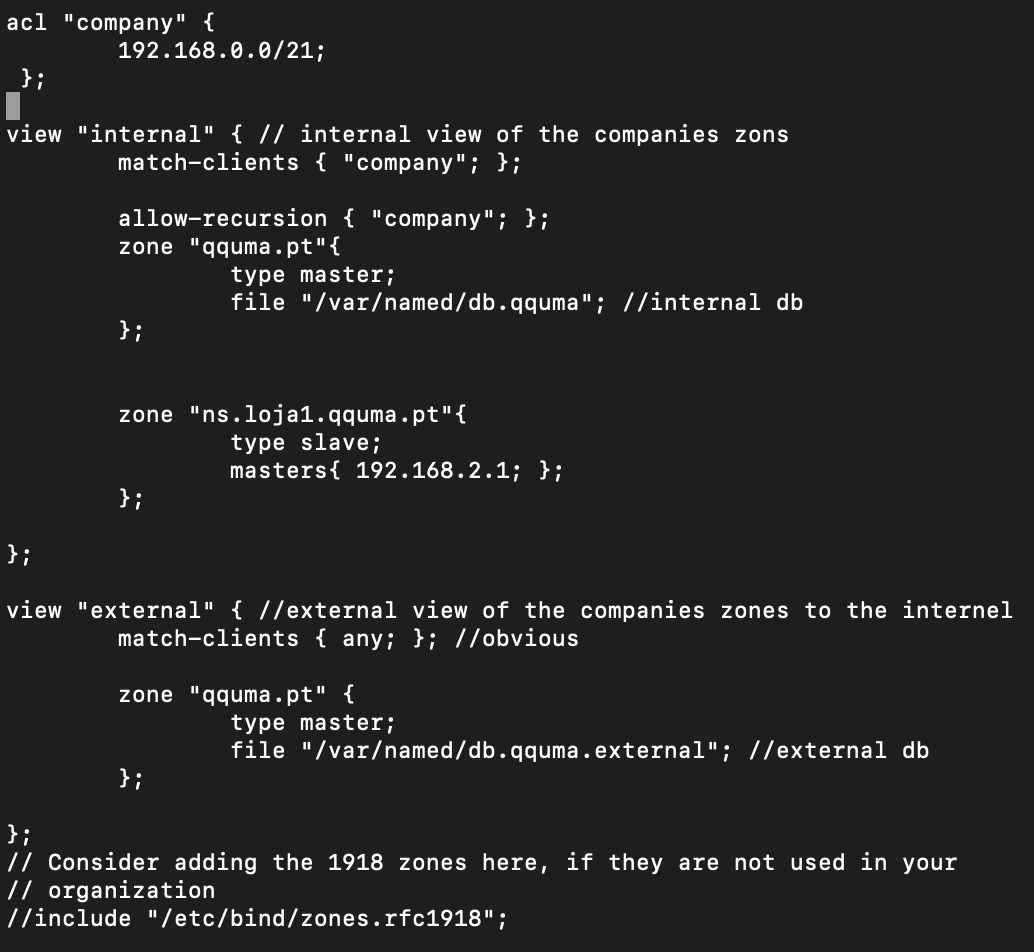
\includegraphics[width=.8\linewidth]{figs/dns_conf/dns_tux13_local.png}
    \caption{Ficheiro named.conf.local Tux13}
    \label{fig:dns_tux13_local}
\end{figure}

Definimos o \textit{range} de IPs 192.168.0.0/21 como pedidos locais e todos os outros como externos.

No ficheiro \textbf{db.qquma}, definimos os \textit{DNS Records} para resolver pedidos internos para os diferentes serviços.

\begin{figure}[H]
    \centering
    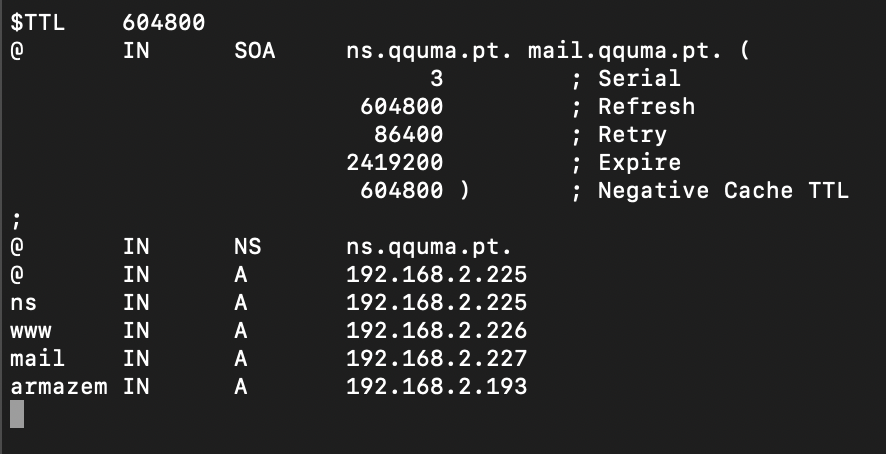
\includegraphics[width=.8\linewidth]{figs/dns_conf/dns_tux13_db_int.png}
    \caption{Ficheiro db.qquma no Tux13}
    \label{fig:dns_tux13_db_int}
\end{figure}

No ficheiro \textbf{db.qquma.external}, definimos os \textit{DNS Records} para resolver pedidos internos para os diferentes serviços.

\begin{figure}[H]
    \centering
    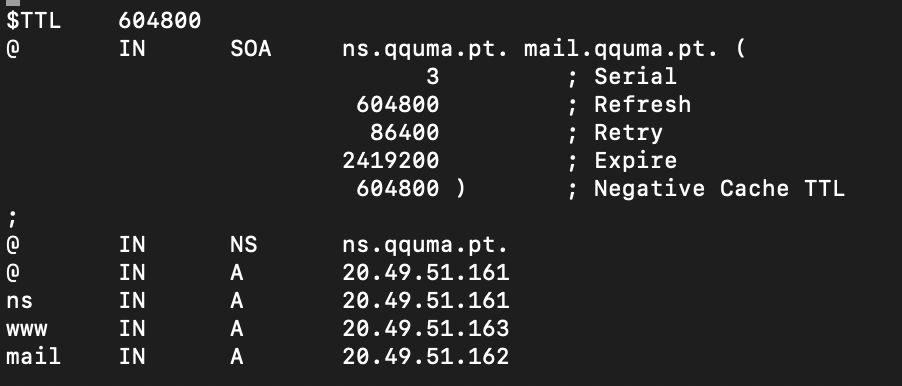
\includegraphics[width=.8\linewidth]{figs/dns_conf/dns_tux13_db_ext.png}
    \caption{Ficheiro db.qquma.external no Tux13}
    \label{fig:dns_tux13_db_ext}
\end{figure}

Por fim, é preciso especificar no ficheiro \verb|/etc/resolv.conf| o servidor DNS que o sistema tem que usar, que neste caso é a si próprio.

\section{Armazém} \label{dns_armazem}

O servidor DNS do armazém tem características diferentes.
Primeiramente, este servidor tem que suportar \textit{Caching}, pelo que essa funcionalidade tem que ser ativada.

Em segundo lugar, o servidor DNS não resolve nenhuma \textit{query}, nem mesmo para si próprio.
Ele tem que reencaminhar os pedidos DNS para a o DNS da rede de servidores, neste caso na \textit{view} interna.
Deste modo, não é preciso configurar um ficheiro \textit{database}, mas é necessário definir o servidor DNS na rede de servidores como \textit{forwarder}.
Isto vai reencaminhar os pedidos que o servidor local não sabe resolver, que neste caso é todos.

\begin{figure}[H]
    \centering
    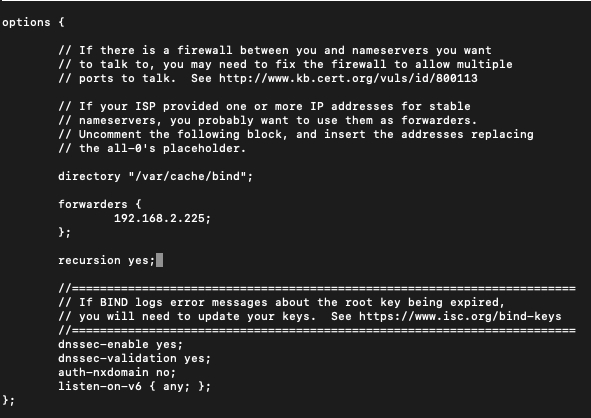
\includegraphics[width=.8\linewidth]{figs/dns_conf/dns_tux12.png}
    \caption{Ficheiro named.conf.options no Tux12}
    \label{fig:dns_tux12}
\end{figure}


\section{Loja} \label{dns_loja}

O servidor DNS da loja tem que conseguir resolver o seu próprio endereço. Deste modo, este servidor DNS é o \textit{slave} do servidor DNS da rede de servidores
Sempre que um \textit{host} pede para resolver o \textit{domain} da loja, o servidor DNS da rede de servidores vai reencaminhar o pedido para este servidor, que o vai resolver.
Note-se que este pedido apenas é redirecionado na \textit{view} interna, isto é, para pedidos locais.
Assim garante-se que o domain não é resolvido para IPs externos..

\begin{figure}[H]
    \centering
    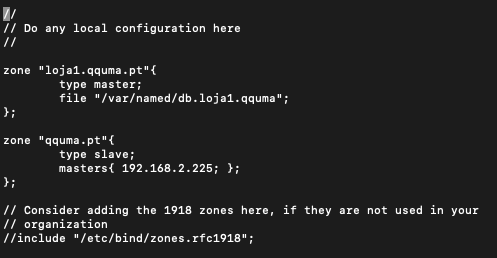
\includegraphics[width=.8\linewidth]{figs/dns_conf/dns_tux14_local.png}
    \caption{Ficheiro named.conf.local no Tux14}
    \label{fig:dns_tux14_local}
\end{figure}

É preciso indicar no ficheiro de configurações qual é a \textit{database} que o DNS tem que aceder para resolver os endereços.

\begin{figure}[H]
    \centering
    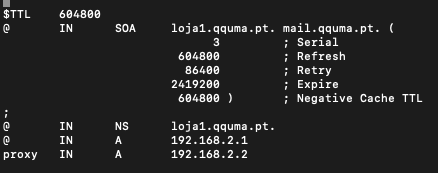
\includegraphics[width=.8\linewidth]{figs/dns_conf/dns_tux14_db.png}
    \caption{Ficheiro db.loja1.qquma no Tux14}
    \label{fig:dns_tux14_db}
\end{figure}

No ficheiro verb|db.loja1.qquma| definimos os \text{DNS Records} quer para o próprio endereço do \textit{Nameserver}, quer para o \textit{Proxy}.